% Copyright 2021 Joel Feldman, Andrew Rechnitzer and Elyse Yeager, except where noted.
% This work is licensed under a Creative Commons Attribution-NonCommercial-ShareAlike 4.0 International License.
% https://creativecommons.org/licenses/by-nc-sa/4.0/

\section*{2.14: Higher Order Derivatives}

\begin{frame}{Table of Contents}
\mapofcontentsB{\bo}
\end{frame}

%----------------------------------------------------------------------------------------
%----------------------------------------------------------------------------------------
\begin{frame}<beamer>
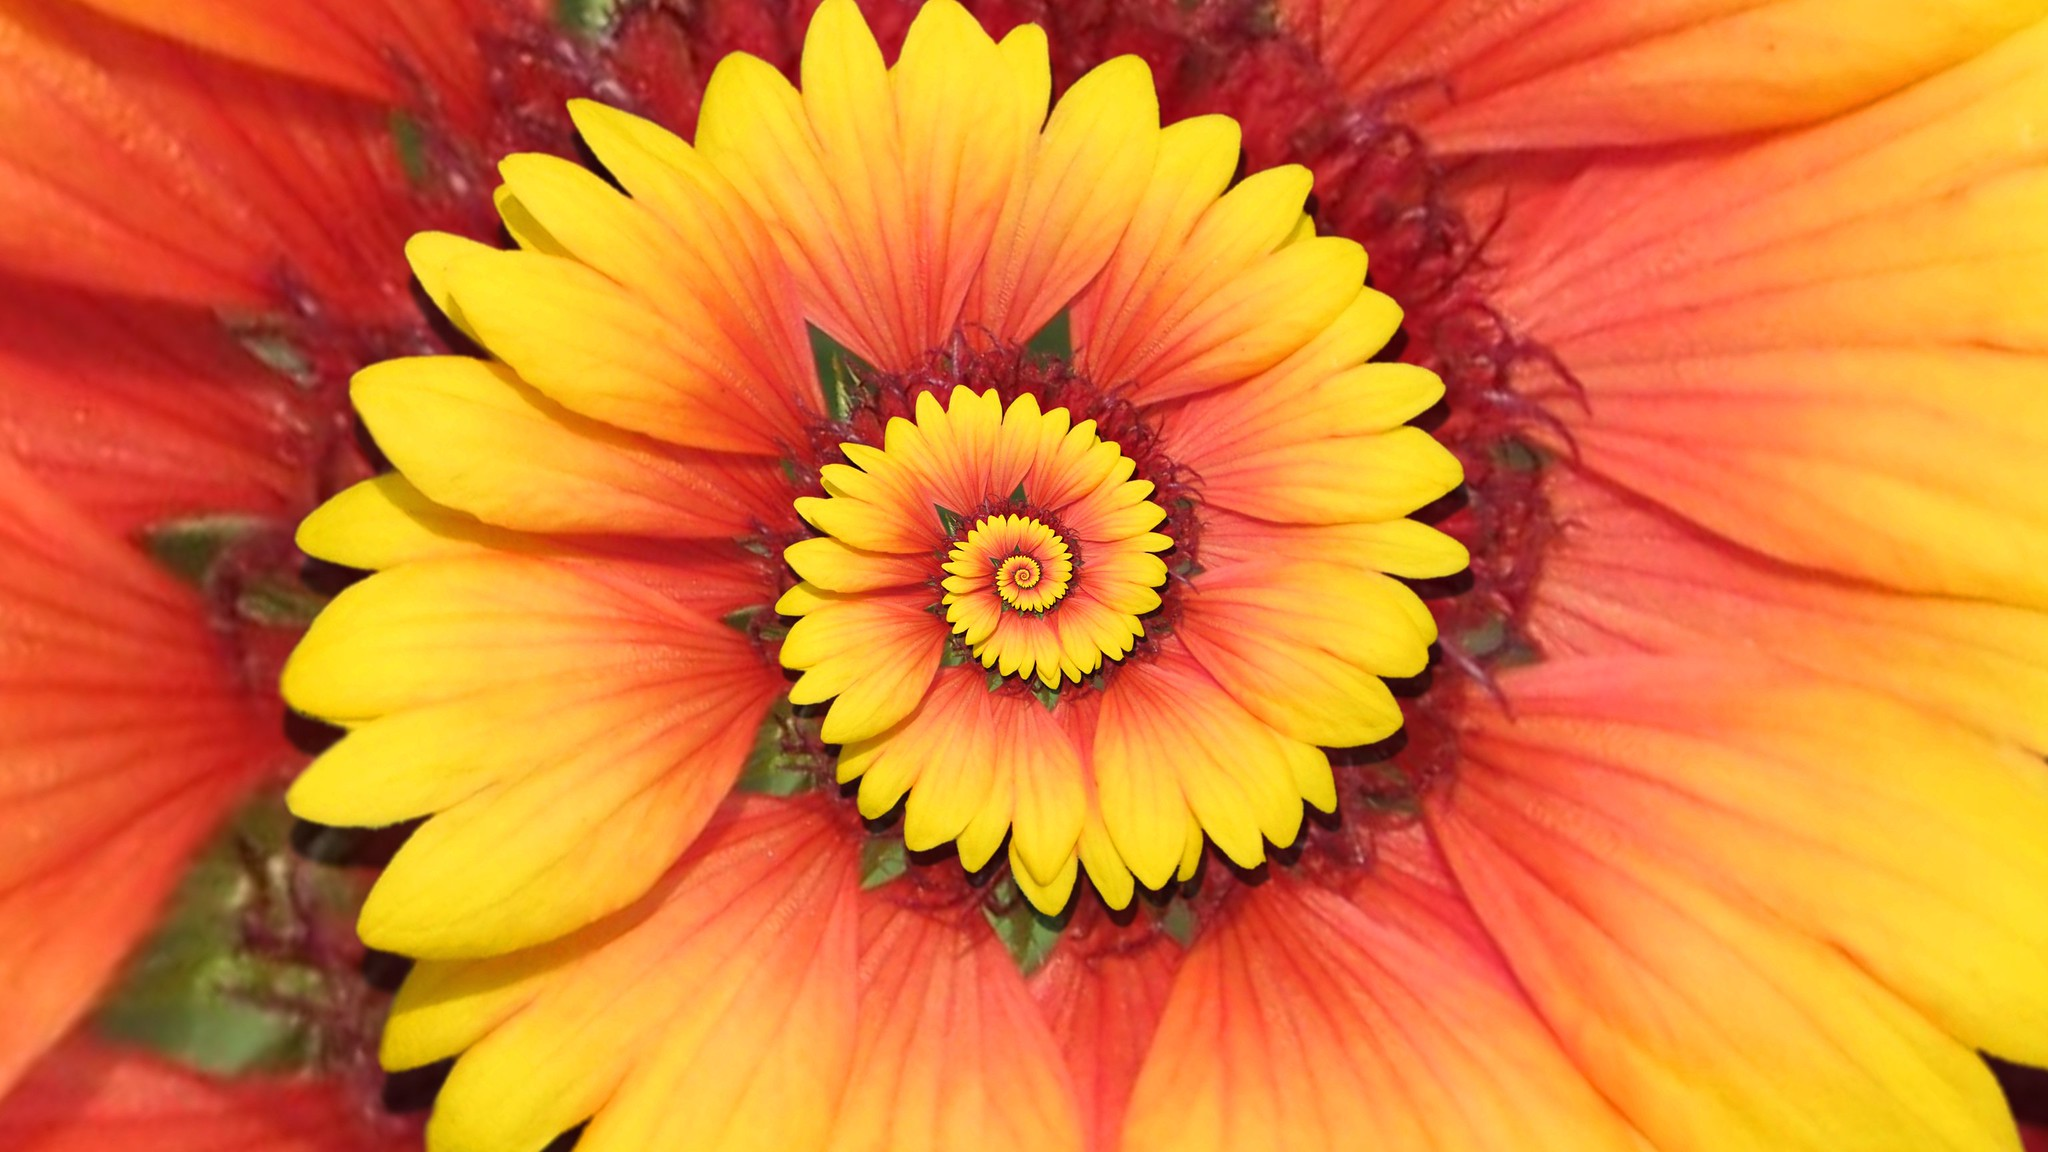
\includegraphics[width=\textwidth]{Clipart/Droste.jpg}
\index{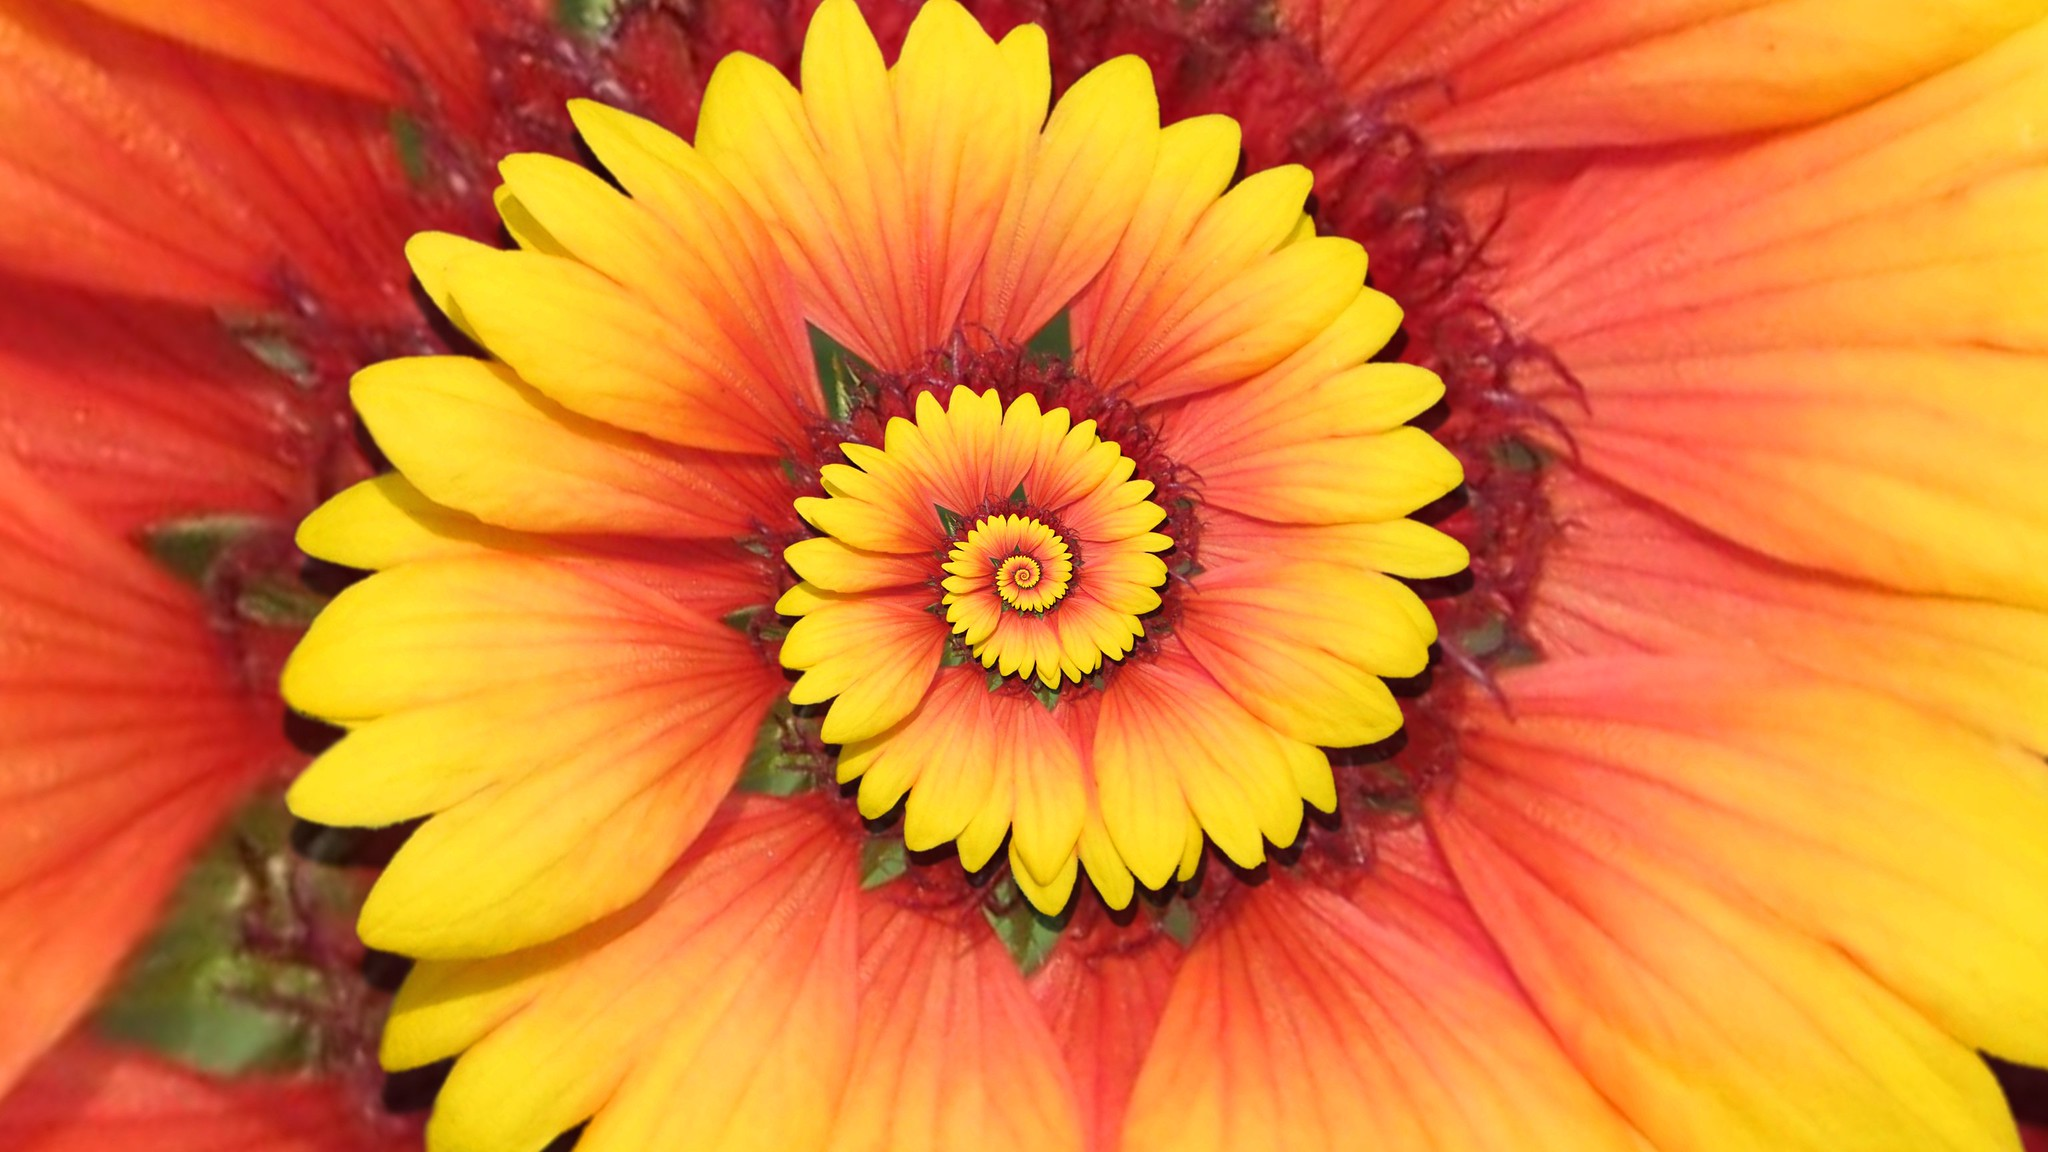
\includegraphics[height=5mm]{Clipart/Droste.jpg}
\href{https://www.flickr.com/photos/gadl/254387060}{`Recursive Blanket Flower'}
by \href{https://www.flickr.com/photos/gadl/}{Alexandre Duret-Lutz} is licensed under
\CCBYNCSAtwo~ 
(accessed 20 July 2021)}
\note{There is something recursive-flavoured about taking derivatives of derivatives, which seemed like a good excuse for a pretty picture. I would have this slide on the projector as students are filing into class as a nice thing to look at. Then I would introduce the lecture as taking derivatives of derivatives, which we could continue for as long as we wanted.}
\end{frame}
%----------------------------------------------------------------------------------------
\begin{frame}[t]{Higher Order Derivatives}
\only<1-2>{\AnswerYes}
\StatusBar{1}{5}
Evaluate $\diff{}{x}\Big[\textcolor{C1}{\diff{}{x}[x^5-2x^2+3]} \Big]$

\pause
\begin{align*}
\color{C1}\diff{}{x}[x^5-2x^2+3] &
\color{C1}=\iftoggle{printsolutions}{5x^4 - 4x}{}\\
\onslide<3-|handout:0>{
\color{M3}\diff{}{x}\left[\textcolor{C1}{\diff{}{x}[x^5-2x^2+3] } \right]&\color{M3}=
\diff{}{x}\left[
\textcolor{C1}{5x^4-4x}
\right]\\
&\color{M3}=20x^3-4}
\end{align*}
\onslide<4->{
\vspace{-5mm}\begin{block}{Notation~\eref{text}{not:higherOrdDeriv}}
The derivative of a derivative is called the \textbf{second derivative}, written 
\[\alert{f''(x)} \qquad\text{or}\qquad 
           \alert{\frac{\text{d}^2y}{\text{d}x^2}(x)}\]
\onslide<5->{Similarly, the derivative of a second derivative is a third derivative, etc.}
\end{block}}
\vfill
\end{frame}
%----------------------------------------------------------------------------------------
%----------------------------------------------------------------------------------------
\begin{frame}[t]
\begin{block}{Notation~\eref{text}{not:higherOrdDeriv}}
\begin{itemize}
\item $f''(x)$ and $f^{(2)}(x)$  and $\ddiff{2}{f}{x}(x)$ all mean
$\diff{}{x}\big(\diff{}{x}f(x)\big)$
\item $f'''(x)$ and $f^{(3)}(x)$  and $\ddiff{3}{f}{x}(x)$ all mean
$\diff{}{x}\big(\diff{}{x}\big(\diff{}{x}f(x)\big)\big)$
\item $f^{(4)}(x)$  and $\ddiff{4}{f}{x}(x)$ both mean
$\diff{}{x}\big(\diff{}{x}\big(\diff{}{x}\big(\diff{}{x}f(x)\big)\big)\big)$
\item and so on.
\end{itemize}
\end{block}
\end{frame}
%----------------------------------------------------------------------------------------
%----------------------------------------------------------------------------------------
\begin{frame}[t]{Typical Example: Acceleration}
\only<3>{\AnswerYes}
\unote{Example~\eref{text}{eg_2_14_1}}
\begin{itemize}
\item Velocity: rate of change of position\pause
\item Acceleration: rate of change of velocity.
\end{itemize}
\pause
The position of an object at time $t$ is given by $s(t) = t(5-t)$. \textit{Time is measured in seconds, and position is measured in metres.}
\begin{enumerate}
\item Sketch the graph giving the position of the object.
\item What is the velocity of the object when $t=1$? Include units.
\item What is the acceleration of the object when $t=1$? Include units.
\end{enumerate}

\only<4|handout:0>{
\begin{center}
\begin{tikzpicture}
\myaxis{t}{.6}{6}{}{.5}{2.5}{t}
\draw[thick, C1] plot[domain=0:5](\x,{\x*(5-\x)/3});
\xcoord{1}{1}
\end{tikzpicture}
\end{center}
}\color{answercolor}
\only<5-|handout:0>{
\begin{align*}
s(t)&=t(5-t)=5t-t^2\\
s'(t)&=5-2t &\onslide<6->{s''(t)&=-2}\\
s'(1)&=5-2(1)=3=\text{vel} & \onslide<6->{-2&=\text{acc}}
\end{align*}
Units of velocity: $\frac{\Delta s}{\Delta t} = \frac{m}{s}$\hfill
Units of acceleration: $\frac{\Delta s'}{\Delta t} = \frac{m/s}{s}=\frac{m}{s^2}$
}
\end{frame}
%----------------------------------------------------------------------------------------
\begin{frame}{Concept Check}
\only<1-2>{\unote{Warning~\eref{text}{warning:dropx}}}
\textbf{True or False:} If $f'(1)=18$, then $f''(1)=0$, \\since the $\diff{}{x}\{18\}=0$.
\iftoggle{printsolutions}{\onslide<2->{\textcolor{answercolor}{\\ False: for example, $f(x) = 9x^2$.}}}{}
\vfill
\begin{multicols}{2}
\only<3->{\unote{Example~\eref{text}{eg:higherOrdDerivA}}
	\textbf{Which of the following is always true of a QUADRATIC polynomial $f(x)$?}
\begin{enumerate}[A.]
\item $f(0)=0$ \iftoggle{printsolutions}{\quad\onslide<4->{\textcolor{answercolor}{$f(x)=ax^2+bx+c$}}}{}
\item $f'(0)=0$\iftoggle{printsolutions}{\quad\onslide<4->{\textcolor{answercolor}{$f'(x)=2ax+b$}}}{}
\item $f''(0)=0$\iftoggle{printsolutions}{\quad\onslide<4->{\textcolor{answercolor}{$f''(x)=2a$}}}{}
\item $f'''(0)=0$\iftoggle{printsolutions}{\quad\onslide<4->{\textcolor{answercolor}{$f'''(x)=0~\checkmark$}}}{}
\item $f^{(4)}(0)=0$\iftoggle{printsolutions}{\quad\onslide<4->{\textcolor{answercolor}{$f^{(4)}(x)=0~\checkmark$}}}{}
\end{enumerate}}
\columnbreak
\onslide<5->{\textbf{Which of the following is always true of a CUBIC polynomial $f(x)$?
}
\begin{enumerate}[A.]
\item $f(0)=0$ \iftoggle{printsolutions}{\onslide<6->{\textcolor{answercolor}{\footnotesize$f(x)=ax^3+bx^2+cx+d$}}}{}
\item $f'(0)=0$\iftoggle{printsolutions}{\only<6->{\textcolor{answercolor}{\quad
     \footnotesize$f'(x)=3ax^2+2bx+c$}}}{}
\item $f''(0)=0$\iftoggle{printsolutions}{\onslide<6->{\textcolor{answercolor}{\quad$f''(x)=6ax+2b$}}}{}
\item $f'''(0)=0$\iftoggle{printsolutions}{\onslide<6->{\textcolor{answercolor}{\quad$f'''(x)=6a$}}}{}
\item $f^{(4)}(0)=0$\iftoggle{printsolutions}{\onslide<6->{\textcolor{answercolor}{\quad$f^{(4)}(x)=0~\checkmark$}}}{}
\end{enumerate}}
\end{multicols}
\only<1>{\QuestionBar{1}{3}\AnswerYes}
\only<2>{\AnswerBar{1}{3}}
\only<3>{\QuestionBar{2}{3}\AnswerYes}
\only<4>{\AnswerBar{2}{3}}
\only<5>{\QuestionBar{3}{3}\AnswerYes}
\only<6>{\AnswerBar{3}{3}}
\end{frame}
%----------------------------------------------------------------------------------------
%----------------------------------------------------------------------------------------
\begin{frame}[t]{Implicit Differentiation}
\unote{Example~\eref{text}{eg:higherOrdDerivC}}
Suppose $y(x)$ is a function such that
\[y(x) = y^3x+x^2-1\]
Find $y''(x)$ at the point $(-2,1)$.
\only<1>{\AnswerYes}
\onslide<2|handout:0>{\color{answercolor}
We start by differentiating both sides of the function. Remember that $y$ is a function, not a variable.
\begin{align*}
y(x)&= y(x)^3 x+x^2+1 \\
\diff{y}{x}(x)&\stackrel{\text{\tiny prod}}{=}y(x)^3+3xy(x)^2\diff{y}{x}(x)+2x \tag{$*$}
\intertext{Let's differentiate both sides again. Remember we have a rule for the product of three functions.}
\ddiff{2}{y}{x}&=3y^2\diff{y}{x}+3\left(y^2\diff{y}{x}+x\cdot 2y\diff{y}{x}\cdot\diff{y}{x}+xy^2\ddiff{2}{y}{x}\right)+2 \tag{$**$}
\end{align*}}
\end{frame}
%----------------------------------------------------------------------------------------
\begin{frame}<beamer>\color{answercolor}\footnotesize
When $x=-2$ and $y=1$, using ($*$), we find
\begin{align*}
\left.\diff{y}{x}\right|_{(-2,1)}
     &=1^3+3(-2)(1^2)\left.\diff{y}{x}\right|_{(-2,1)}+2(-2)
       =-3-6\left.\diff{y}{x}\right|_{(-2,1)}\\
\left.\diff{y}{x}\right|_{(-2,1)}&=-\frac37
\intertext{We set $x=-2$, $y=1$, and $\diff{y}{x}=-\frac37$ in  equation ($**$). Now by \alert{$\ddiff{2}{y}{x}$}, we actually mean \alert{$\left.\ddiff{2}{y}{x}\right|_{(-2,1)}$}, but to avoid clutter we don't write it that way until the end.}
\ddiff{2}{y}{x}&=3(1)\left(-\frac37\right)+3\left((1)\left(-\frac37\right)+(-2)\cdot 2(1)\left(-\frac37\right)\cdot\left(-\frac37\right)+(-2)(1)\ddiff{2}{y}{x}\right)+2 \\
&=-\frac97+3\left(-\frac37-\frac{36}{49}-2\ddiff{2}{y}{x}\right)+2\\
&=\left(2-\frac{18}{7}-\frac{108}{49}\right)-6\ddiff{2}{y}{x}\\
7\ddiff{2}{y}{x}&=-\frac{136}{7^2}\\
\left.\ddiff{2}{y}{x}\right|_{(-2,1)}&=-\frac{136}{7^3}
\end{align*}

\end{frame}
 %----------------------------------------------------------------------------------------
%----------------------------------------------------------------------------------------
%----------------------------------------------------------------------------------------
